\documentclass[11pt]{beamer}
\usepackage{tikz, stackengine}
\usetikzlibrary{decorations.text}
\usetikzlibrary{shapes}
\usetikzlibrary{overlay-beamer-styles}
\usetikzlibrary{matrix}
% \usepackage{pgfpages}
% \pgfpagesuselayout{4 on 1}[a4paper,border shrink=5mm,landscape]

\tikzset{
  every overlay node/.style={
    % draw=black,fill=white,rounded corners,anchor=north west,
  },
}
% Usage:
% \tikzoverlay at (-1cm,-5cm) {content};
% or
% \tikzoverlay[text width=5cm] at (-1cm,-5cm) {content};

\def\tikzoverlay{%
   \tikz[baseline,overlay]\node[every overlay node]
}%



\newcommand{\tikzmark}[1]{\tikz[overlay,remember picture] \node (#1) {};}

\newcommand*{\LabelText}[3]{%
\tikzmark{a}#1\tikzmark{b}%
\begin{tikzpicture}[overlay,remember picture]
    \path (a.north) -- (b.north) node [yshift=3.0ex, midway,rectangle,draw=#3,rounded corners=2pt,inner sep=1pt,fill=-#3]  {#2\strut};
\end{tikzpicture}%
}

\newcommand*{\bubbleHere}[1]{\LabelText{#1}{noun}{red}}

\tikzstyle{rect3} = [rectangle, minimum width=3cm, minimum height=1cm, text centered, text width=3cm, draw=black]
\tikzstyle{rect4} = [rectangle, minimum width=3cm, minimum height=1cm, text centered, text width=3cm, draw=red]


\usetheme{Frankfurt}
\useinnertheme{rectangles}

\usecolortheme{lily}
\useoutertheme[section= false,subsection=false]{miniframes}
\usefonttheme{serif}

\title{Basic Trigonometric Identities and Equations}

\begin{document}

\begin{frame}
\tikzoverlay at (9cm,0cm) {
\includegraphics{lion}};
\titlepage
\end{frame}



\begin{frame}

\textcolor{red}{Quotient Identities}
\begin{columns}
\column{0.5\textwidth}
$$\mathbf{tan\theta=\frac{ sin\theta}{ sin\theta}} $$
\column{0.5\textwidth}
$$\mathbf{tan\theta=\frac{ sin\theta}{ sin\theta}} $$

\end{columns}

\textcolor{red}{Reciprocal Identities}
\begin{columns}
\column{0.33\textwidth}
$$\mathbf{tan\theta=\frac{ sin\theta}{ sin\theta}} $$
\column{0.33\textwidth}
$$\mathbf{tan\theta=\frac{ sin\theta}{ sin\theta}} $$
\column{0.33\textwidth}
$$\mathbf{tan\theta=\frac{ sin\theta}{ sin\theta}} $$
\end{columns}

\textcolor{red}{Reciprocal Identities}
\begin{columns}
\column{0.33\textwidth}
$$\mathbf{tan\theta=\frac{ sin\theta}{ sin\theta}} $$
\column{0.33\textwidth}
$$\mathbf{tan\theta=\frac{ sin\theta}{ sin\theta}} $$
\column{0.33\textwidth}
$$\mathbf{tan\theta=\frac{ sin\theta}{ sin\theta}} $$
\end{columns}

\end{frame}


\begin{frame}

\frametitle{Do you remember the Unit Circle?}


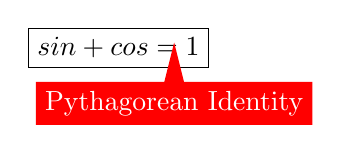
\begin{tikzpicture}

\node(A)[draw]{$sin + cos = 1$};

\node[rectangle callout,color=white, fill=red,  callout relative pointer={(0,0.5)},below right of= A]  {Pythagorean Identity}; 
     
\end{tikzpicture}
\end{frame}

\begin{frame}
\frametitle{Simply Each Expression}


\begin{columns}
\begin{column}{0.25\textwidth}
Lorem ipsum dolor sit amet, consectetur adipisicing elit, sed do eiusmod tempor incididunt ut labore et dolore magna aliqua.
\end{column}
\textcolor{blue}{\vrule{}}
\begin{column}{0.375\textwidth}
Lorem ipsum dolor sit amet, consectetur adipisicing elit, sed do eiusmod tempor incididunt ut labore et dolore magna aliqua
\end{column}
\vrule{}
\begin{column}{0.375\textwidth}
Lorem ipsum dolor sit amet, consectetur adipisicing elit, sed do eiusmod tempor incididunt ut labore et dolore magna aliqua.
\end{column}
\end{columns}
\end{frame}

\begin{frame}
\label{columns}
\frametitle{Example}

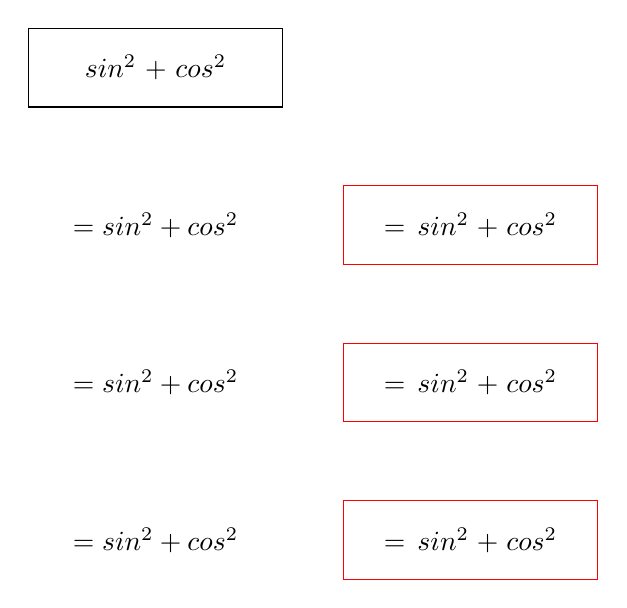
\begin{tikzpicture}[node distance=4cm]

\node(line1)[rect3]{$sin^{2} + cos^{2} $};
\node(line2)[rectangle, below of = line1, node distance = 2cm]{$ = sin^{2} + cos^{2} $};
\node(line3)[rectangle, below of = line2,  node distance = 2cm]{$ = sin^{2} + cos^{2} $};
\node(line4)[rectangle, below of = line3,  node distance = 2cm]{$ = sin^{2} + cos^{2} $};
\node(line5)[rect4, right of = line2]{$ = sin^{2} + cos^{2} $};
\node(line6)[rect4, right of = line3]{$ = sin^{2} + cos^{2} $};
\node(line7)[rect4, right of = line4]{$ = sin^{2} + cos^{2} $};
  
  
\end{tikzpicture}
 
    
\end{frame}


\begin{frame}{RED TABLEEEEE}
% \begin{onlyenv}<+->
\begin{onlyenv}<+->
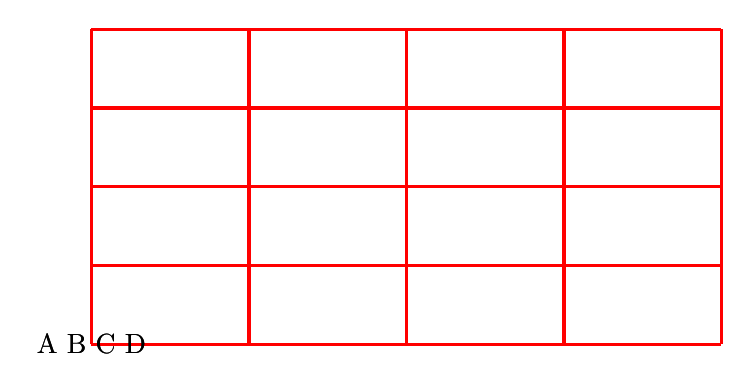
\begin{tikzpicture}
\draw[xstep=2cm,ystep=1,red,very thick] (0,0) grid (8,4);



\node[visible on=<1->]  at  (0,0){A B C D};

\node[visible on=<2->]  at  (0,0){A B C D};



\end{tikzpicture}

\end{onlyenv}
% \end{onlyenv}
\end{frame}

\begin{frame}{RED TABLE!!!}
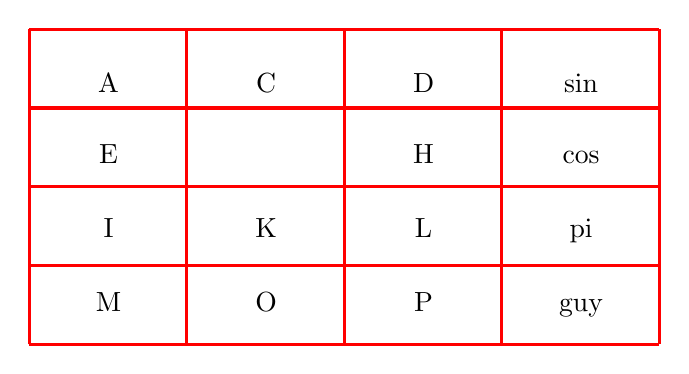
\begin{tikzpicture}
\draw[xstep=2cm,ystep=1,red,very thick] (0,0) grid (8,4);
% \draw[<->] (0,0) -- (4,4);

\matrix[matrix of nodes,
inner sep=0pt,
anchor=south west,
nodes={inner sep=0pt,text width=2cm,align=center,minimum height=0.9cm}
]{
A && C && D && sin\\
E &&  && H && cos\\
I && K && L && pi\\
M && O && P && guy\\
};

\end{tikzpicture}
    
\end{frame}

\begin{frame}{ASS TO ASS}
    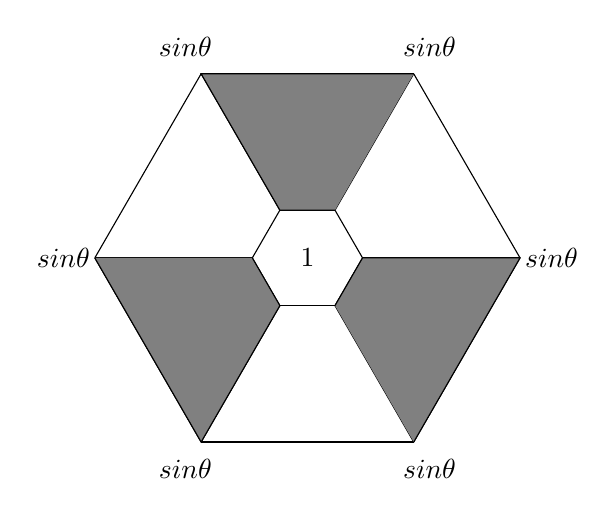
\begin{tikzpicture}
       \newdimen\R
   \R=2.7cm
   
    \newdimen\r
   \r=0.7cm
%   \draw (0:\R) \foreach \x in {60,120,...,360} {  -- (\x:\R) };
\node[rectangle]{1};
\foreach \x in {60,120,...,360}{
    \draw (\x:\R)  --  (\x+60:\R) ;
    \draw (\x:\r)  --  (\x+60:\r) ;
    \draw (\x:\r)  --  (\x:\R);
    
    };
    
   \node  at (60:3.1cm){$sin\theta$};
    \node  at (120:3.1cm){$sin\theta$};
    \node  at (180:3.1cm){$sin\theta$};
    \node  at (240:3.1cm){$sin\theta$};
    \node  at (300:3.1cm){$sin\theta$};
    \node  at (360:3.1cm){$sin\theta$};
    
  \foreach \x in {60, 180, 300}{
    \draw[fill=gray] (\x:\r)--(\x+60:\r)--(\x+60:\R)--(\x:\R);
  };
    \end{tikzpicture}
\end{frame}
\end{document}